\documentclass{standalone}

\usepackage[english]{babel} % English language/hyphenation
\usepackage{clock} % Required for generation clock icon
\ClockFrametrue\ClockStyle=3 % Format the clock icons
\usepackage{gensymb} % gives the degree symbol
\usepackage{graphicx} % Required for including pictures
\usepackage{tikz} % Required for drawing custom shapes
\usetikzlibrary{arrows}
\usetikzlibrary{arrows.meta}
\usetikzlibrary{shapes.misc}
\usetikzlibrary{decorations.pathreplacing}

\definecolor{gridgray}{RGB}{192,192,192}
\definecolor{medgray}{RGB}{128,128,128}
\definecolor{redback}{RGB}{255,168,168}
\definecolor{redback2}{RGB}{128,0,0}
\definecolor{greenback}{RGB}{168,255,168}
\definecolor{greenpastel}{RGB}{210,255,210}
\definecolor{greenback2}{RGB}{0,192,0}
\definecolor{darkgreenback}{RGB}{0,96,0}
\definecolor{yellowback}{RGB}{255,255,168}
\definecolor{darkyellowback}{RGB}{96,96,0}
\definecolor{orangeback}{RGB}{255,192,128}
\definecolor{orangeback2}{RGB}{255,220,192}
\definecolor{darkorangeback}{RGB}{192,96,0}
\definecolor{yellowback2}{RGB}{255,255,192}
\definecolor{aquaback}{RGB}{192,255,255}
\definecolor{darkaquaback}{RGB}{0,96,96}
\definecolor{blueback}{RGB}{168,168,255}
\definecolor{magentaback}{RGB}{255,210,255}
\definecolor{darkmagentaback}{RGB}{96,0,96}
\definecolor{unusedgray}{RGB}{192,192,192}

\begin{document}
    \rotatebox{315}{%
	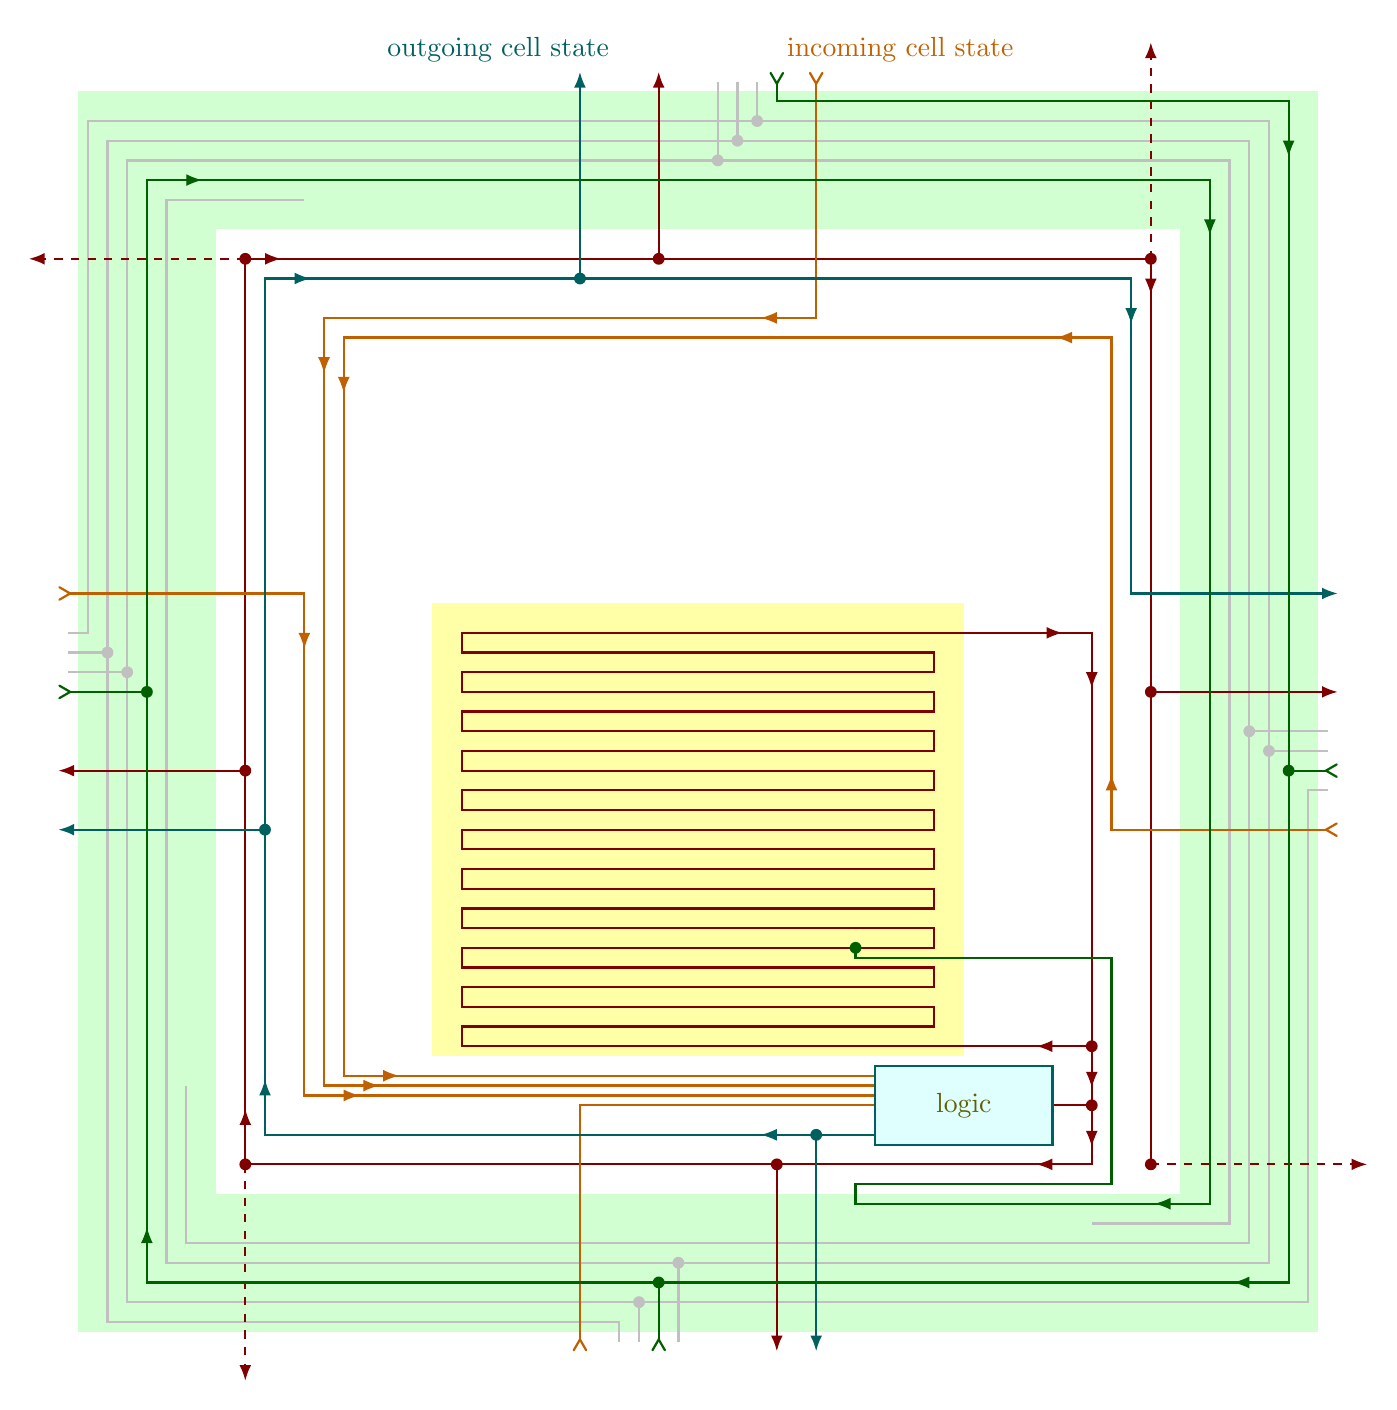
\begin{tikzpicture}[scale=0.25]%
%		Corner dots
%		\fill[fill=black] (0,0) circle (0.3);
%		\fill[fill=black] (64,0) circle (0.3);
%		\fill[fill=black] (0,64) circle (0.3);
%		\fill[fill=black] (64,64) circle (0.3);


                % shell, kernel, and nucleus
                \fill[greenpastel] ( 0.5,  0.5) rectangle (63.5, 63.5);
                \fill[white]       ( 7.5,  7.5) rectangle (56.5, 56.5);
                \fill[yellowback]  (18.5, 14.5) rectangle (45.5, 37.5);


		% Grey (unused) wires
		\draw[unusedgray,thick] (0,36) -- (1,36) -- (1,62) -- (61,62) -- (61,4) -- (5,4) -- (5,58) -- (12,58);
		\draw[unusedgray,thick] (0,35) -- (2,35);
		\draw[unusedgray,thick] (0,34) -- (3,34);
		\draw[unusedgray,thick] (35,64) -- (35,62);
		\draw[unusedgray,thick] (34,64) -- (34,61);
		\draw[unusedgray,thick] (33,64) -- (33,60);
		\draw[unusedgray,thick] (64,28) -- (63,28) -- (63,2) -- (3,2) -- (3,60) -- (59,60) -- (59,6) -- (52,6);
		\draw[unusedgray,thick] (28,0) -- (28,1) -- (2,1) -- (2,61) -- (60,61) -- (60,5) -- (6,5) -- (6,13);
		\draw[unusedgray,thick] (64,31) -- (60,31);
		\draw[unusedgray,thick] (64,30) -- (61,30);
		\draw[unusedgray,thick] (29,0) -- (29,2);
		\draw[unusedgray,thick] (31,0) -- (31,4);

		\fill[fill=unusedgray] (35,62) circle (0.3);
		\fill[fill=unusedgray] (34,61) circle (0.3);
		\fill[fill=unusedgray] (33,60) circle (0.3);

		\fill[fill=unusedgray] (61,30) circle (0.3);
		\fill[fill=unusedgray] (60,31) circle (0.3);

		\fill[fill=unusedgray] (29,2) circle (0.3);
		\fill[fill=unusedgray] (31,4) circle (0.3);

		\fill[fill=unusedgray] (3,34) circle (0.3);
		\fill[fill=unusedgray] (2,35) circle (0.3);
		
		% Red wires
		\draw[redback2,thick] (50,12) -- (52,12) -- (52,15) -- (20,15) -- (20,16) -- (44,16) -- (44,17) -- (20,17) -- (20,18) -- (44,18) -- (44,19) -- (20,19) -- (20,20) -- (44,20) -- (44,21) -- (20,21) -- (20,22) -- (44,22) -- (44,23) -- (20,23) -- (20,24) -- (44,24) -- (44,25) -- (20,25) -- (20,26) -- (44,26) -- (44,27) -- (20,27) -- (20,28) -- (44,28) -- (44,29) -- (20,29) -- (20,30) -- (44,30) -- (44,31) -- (20,31) -- (20,32) -- (44,32) -- (44,33) -- (20,33) -- (20,34) -- (44,34) -- (44,35) -- (20,35) -- (20,36) -- (52,36) -- (52,15);
		\draw[redback2,thick,-{Latex[length=2mm,width=1.5mm]}] (52,12) -- (52,9) -- (36,9) -- (36,-0.5);
		\draw[redback2,thick,-{Latex[length=2mm,width=1.5mm]}] (36,9) -- (9,9) -- (9,29) -- (-0.5,29);
		\draw[redback2,thick,-{Latex[length=2mm,width=1.5mm]}] (9,29) -- (9,55) -- (30,55) -- (30,64.5);
		\draw[redback2,thick,-{Latex[length=2mm,width=1.5mm]}] (30,55) -- (55,55) -- (55,33) -- (64.5,33);
        \draw[redback2,thick] (55,33) -- (55,9);
		\draw[redback2,-{Latex[length=2mm,width=1.5mm]}] (48,36) -- (50.5,36);
		\draw[redback2,-{Latex[length=2mm,width=1.5mm]}] (52,35) -- (52,33.2);
		\draw[redback2,-{Latex[length=2mm,width=1.5mm]}] (51,15) -- (49.2,15);
		\draw[redback2,-{Latex[length=2mm,width=1.5mm]}] (52,15) -- (52,12.9);
		\draw[redback2,-{Latex[length=2mm,width=1.5mm]}] (52,12) -- (52,9.9);
		\draw[redback2,-{Latex[length=2mm,width=1.5mm]}] (51,9) -- (49.2,9);
		\draw[redback2,-{Latex[length=2mm,width=1.5mm]}] (9,10) -- (9,11.8);
		\draw[redback2,-{Latex[length=2mm,width=1.5mm]}] (9,55) -- (10.8,55);
		\draw[redback2,-{Latex[length=2mm,width=1.5mm]}] (55,55) -- (55,53.2);
		\fill[fill=redback2] (52,15) circle (0.3);
		\fill[fill=redback2] (52,12) circle (0.3);
		\fill[fill=redback2] (36,9) circle (0.3);
		\fill[fill=redback2] (9,29) circle (0.3);
		\fill[fill=redback2] (30,55) circle (0.3);
		\fill[fill=redback2] (55,33) circle (0.3);
		
		\fill[fill=redback2] (55,9) circle (0.3);
		\fill[fill=redback2] (9,9) circle (0.3);
		\fill[fill=redback2] (55,55) circle (0.3);
		\fill[fill=redback2] (9,55) circle (0.3);

        % Construction arms
		\draw[redback2,dashed,thick,-{Latex[length=2mm,width=1.5mm]}] (55,9) -- (66, 9);
		\draw[redback2,dashed,thick,-{Latex[length=2mm,width=1.5mm]}] (55,55) -- (55, 66);
		\draw[redback2,dashed,thick,-{Latex[length=2mm,width=1.5mm]}] (9, 55) -- (-2, 55);
		\draw[redback2,dashed,thick,-{Latex[length=2mm,width=1.5mm]}] (9, 9) -- (9, -2);
		
		% Orange wires
		\draw[darkorangeback,thick,{angle 60 reversed[length=2mm,width=1.5mm]}-] (26,-0.5) -- (26,12) -- (41,12);
		
		\draw[darkorangeback,thick,{angle 60 reversed[length=2mm,width=1.5mm]}-] (-0.5,38) -- (12,38) -- (12,12.5) -- (41,12.5);
		\draw[darkorangeback,-{Latex[length=2mm,width=1.5mm]}] (12,37) -- (12,35.2);
		\draw[darkorangeback,-{Latex[length=2mm,width=1.5mm]}] (13,12.5) -- (14.8,12.5);
		
		\draw[darkorangeback,thick,{angle 60 reversed[length=2mm,width=1.5mm]}-] (38,64.5) node[anchor=south west,shift={(-0.5,0)}]{incoming cell state} -- (38,52) -- (13,52) -- (13,13) -- (41,13);
		\draw[darkorangeback,-{Latex[length=2mm,width=1.5mm]}] (37,52) -- (35.2,52);
		\draw[darkorangeback,-{Latex[length=2mm,width=1.5mm]}] (13,51) -- (13,49.2);
		\draw[darkorangeback,-{Latex[length=2mm,width=1.5mm]}] (14,13) -- (15.8,13);
		
		\draw[darkorangeback,thick,{angle 60 reversed[length=2mm,width=1.5mm]}-] (64.5,26) -- (53,26) -- (53,51) -- (14,51) -- (14,13.5) -- (41,13.5);
		\draw[darkorangeback,-{Latex[length=2mm,width=1.5mm]}] (53,27) -- (53,28.8);
		\draw[darkorangeback,-{Latex[length=2mm,width=1.5mm]}] (52,51) -- (50.2,51);
		\draw[darkorangeback,-{Latex[length=2mm,width=1.5mm]}] (14,50) -- (14,48.2);
		\draw[darkorangeback,-{Latex[length=2mm,width=1.5mm]}] (15,13.5) -- (16.8,13.5);
		
		
		% Aqua wires
		\draw[darkaquaback,thick,-{Latex[length=2mm,width=1.5mm]}] (41,10.5) -- (38,10.5) -- (38,-0.5);
		\draw[darkaquaback,thick,-{Latex[length=2mm,width=1.5mm]}] (38,10.5) -- (10,10.5) -- (10,54) -- (26,54) -- (26,64.5) node[anchor=south east,shift={(0.5,0)}]{outgoing cell state};
		\draw[darkaquaback,thick,-{Latex[length=2mm,width=1.5mm]}] (26,54) -- (54,54) -- (54,38) -- (64.5,38);
		\draw[darkaquaback,thick,-{Latex[length=2mm,width=1.5mm]}] (10,26) -- (-0.5,26);
		\fill[fill=darkaquaback] (38,10.5) circle (0.3);
		\fill[fill=darkaquaback] (26,54) circle (0.3);
		\fill[fill=darkaquaback] (10,26) circle (0.3);
		\draw[darkaquaback,-{Latex[length=2mm,width=1.5mm]}] (37,10.5) -- (35.2,10.5);
		\draw[darkaquaback,-{Latex[length=2mm,width=1.5mm]}] (10,11.5) -- (10,13.3);
		\draw[darkaquaback,-{Latex[length=2mm,width=1.5mm]}] (10,54) -- (12.3,54);
		\draw[darkaquaback,-{Latex[length=2mm,width=1.5mm]}] (54,53.5) -- (54,51.7);
		
		
		% Green wires
		\draw[darkgreenback,thick,{angle 60 reversed[length=2mm,width=1.5mm]}-] (36,64.5) -- (36,63) -- (62,63) -- (62,29);
		\draw[darkgreenback,thick,{angle 60 reversed[length=2mm,width=1.5mm]}-] (64.5,29) -- (62,29) -- (62,3) -- (30,3);
		\draw[darkgreenback,thick,{angle 60 reversed[length=2mm,width=1.5mm]}-] (30,-0.5) -- (30,3) -- (4,3) -- (4,33);
		\draw[darkgreenback,thick,{angle 60 reversed[length=2mm,width=1.5mm]}-] (-0.5,33) -- (4,33) -- (4,59) -- (58,59) -- (58,7) -- (40,7) -- (40,8) -- (53,8) -- (53,19.5) -- (40,19.5) -- (40,20);
		\fill[fill=darkgreenback] (62,29) circle (0.3);
		\fill[fill=darkgreenback] (30,3) circle (0.3);
		\fill[fill=darkgreenback] (4,33) circle (0.3);
		\fill[fill=darkgreenback] (40,20) circle (0.3);
		\draw[darkgreenback,-{Latex[length=2mm,width=1.5mm]}] (62,62) -- (62,60.2);
		\draw[darkgreenback,-{Latex[length=2mm,width=1.5mm]}] (61,3) -- (59.2,3);
		\draw[darkgreenback,-{Latex[length=2mm,width=1.5mm]}] (4,4) -- (4,5.8);
		\draw[darkgreenback,-{Latex[length=2mm,width=1.5mm]}] (5,59) -- (6.8,59);
		\draw[darkgreenback,-{Latex[length=2mm,width=1.5mm]}] (58,58) -- (58,56.2);
		\draw[darkgreenback,-{Latex[length=2mm,width=1.5mm]}] (57,7) -- (55.2,7);
		
		
		% LOGIC component
		\filldraw[thick,color=darkaquaback,fill=aquaback!50] (41,10) -- (50,10) -- (50,14) -- (41,14) -- cycle;
		\draw[darkyellowback] (45.5,12) node {logic};
		
%		BORDER
%		\draw[gridgray] (-1,-1) rectangle (65,67);
	\end{tikzpicture}
    }
\end{document}
